\documentclass[12pt,a4paper]{article}
\usepackage[utf8]{inputenc}
\usepackage[MeX]{polski}
\usepackage{indentfirst} 
\usepackage{graphicx}
\usepackage{geometry}
\usepackage{lipsum}
\usepackage{latexsym, amsmath, amssymb, amsthm}

\frenchspacing
%\linespread{1.5}

\author{Almuludek}
\title{Bawimy się \LaTeX em}
\date{Załęcze Wielkie, \today}

\begin{document}
\maketitle

\section{Zaczynamy!}
Witaj, drogi almuludku! Jestem Twoim pierwszym plikiem w \LaTeX u. % Jestem komentarzem!
Jest \emph{bardzo ważne}, żebyś zrozumiał wszystkie użyte we mnie komendy. Możesz mnie dowolnie edytować i patrzeć, co się będzie działo. 
Przed tym zdaniem był enter, ale nic się nie stało. 

A przed tym były dwa i \ldots mamy nowy akapit! \par A teraz następny, a w nim dużo spacji:                        których wcale nie widać.

\subsection{Wyświetl mnie!}

\begin{itemize}
\item Poniżej w komentarzu komenda z pierwszej linijki tego pliku. Usuń znak komentarza (\texttt{\%}) i spróbuj sformatować ją tak, żeby wyświetlała się jak w ściądze. 
%\documentclass[12pt,a4paper]{article}
\item Tak naprawdę należałoby zrobić to inaczej (przy pomocy otoczenia \texttt{verbatim}), ale to niezłe ćwiczenie na kroje pisma i znaki specjalne.

\item A potem coś 
\begin{enumerate}
\item pogrub, \item pochyl, \item napisz kapitalikami \item lub czcionką o bezszeryfową.
\end{enumerate}

\item Albo nawet spróbuj zrobić kilka z tych rzeczy na raz.
\end{itemize}

\subsection{Napraw mnie!}

Na obozie Klubu Astronomicznego "Almukantarat", który odbył się w dniach 2 - 16 sierpnia 2016r w Załęczu Wielkim, wydarzyło się coś niesamowitego... Na namiot komendanta spadł-nagle i niespodziewanie- ogromny różowo -- złoty meteoryt o temperaturze -20 $^\circ C$.

\section{Trochę matematyki}

Na początek napiszmy jakieś proste ułamki:
\begin{equation}
\frac{1}{2} - \frac{1}{3} = \frac{1}{6}
\end{equation}

Teraz spróbuj sobie przypomnieć (albo poznać) i zapisać twierdzenie Leibniza-Newtona? A potem sprawdź, jak wyglądałoby ono umieszczone pomiędzy dolarami, zamiast w środowisku \texttt{equation}. 

Czas na trochę fizyki. Na pewno znacie prawo Coulomba:
\begin{equation}
\vec{F} = k \frac{q Q}{r^2}\hat{r}, \qquad \mbox{gdzie:} \qquad k = \frac{1}{4 \pi \epsilon_0} = 8{,}99 \cdot 10^9~\mathrm{\frac{N \cdot m^2}{C^2}}
\end{equation}
Zwróć uwagę na formatowanie!

A teraz pobaw się jeszcze chwilę różnymi wyrażeniami matematycznymi. 

\section{A może wstawkę?}

Oto prosta tabelka:

\begin{tabular}{|lc|r|} \hline
Wszyscy & zginiemy & sialalalala \\
Bolesną  & śmiercią & sialalalalala \\
\end{tabular}
Napraw ją tak, żeby miała narysowane wszystkie możliwe krawędzie. Potem umieść ją w otoczeniu \texttt{table} i popatrz, co się zmieni. 

\begin{figure}
\begin{center}
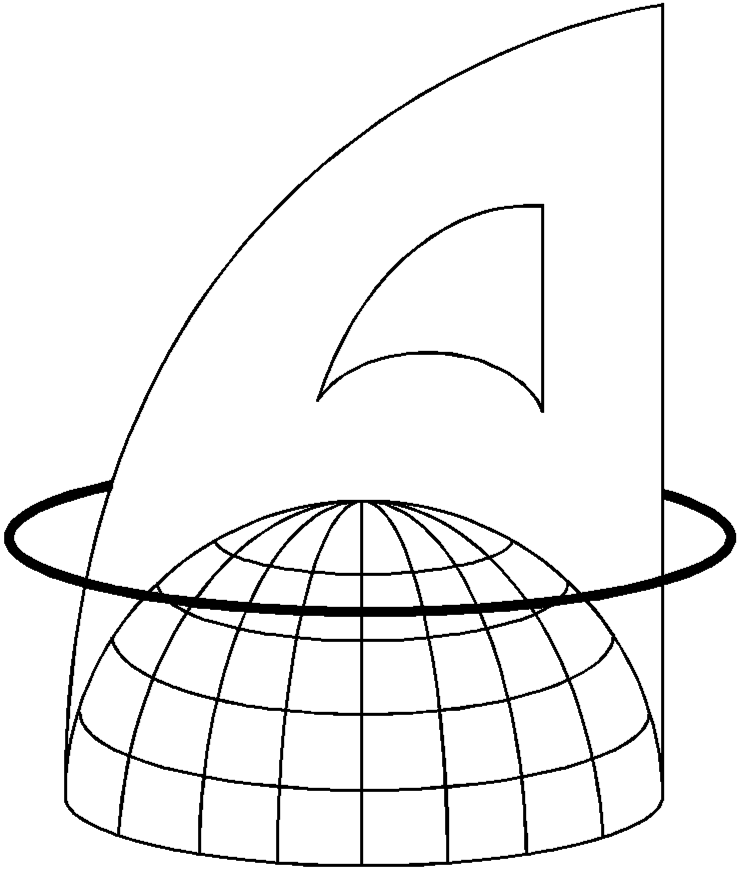
\includegraphics[width=0.2\textwidth]{logo.png}
\end{center}
\caption{\label{logo} A cóż to?}
\end{figure}

\begin{figure}[h]
\begin{flushleft}
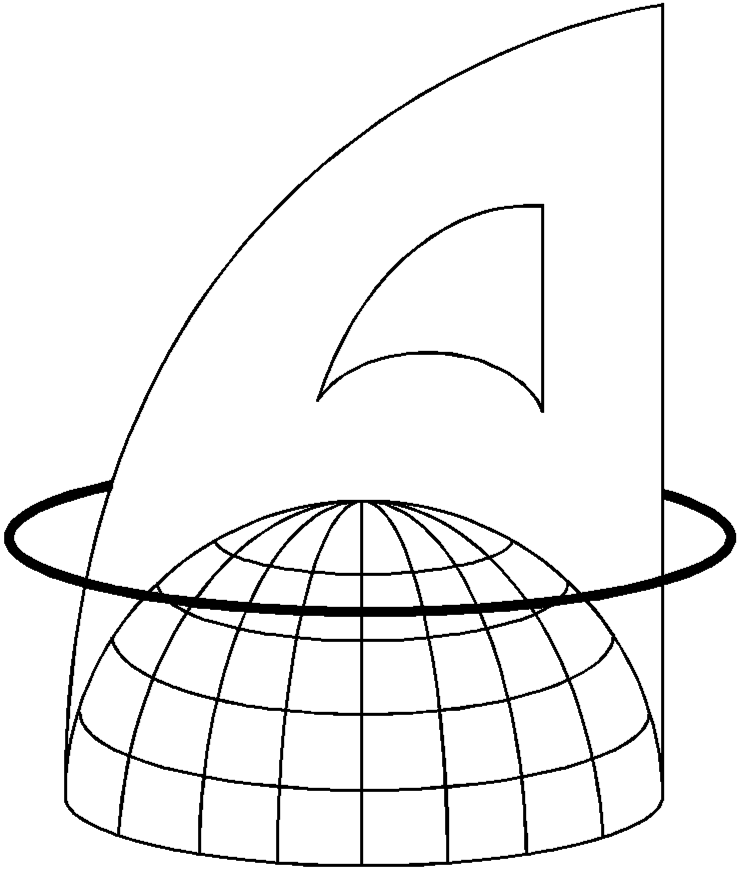
\includegraphics[width=0.3\textwidth]{logo.png}
\end{flushleft}
\caption{\label{almu} A to?}
\end{figure}

\begin{figure}[p]
\begin{flushright}
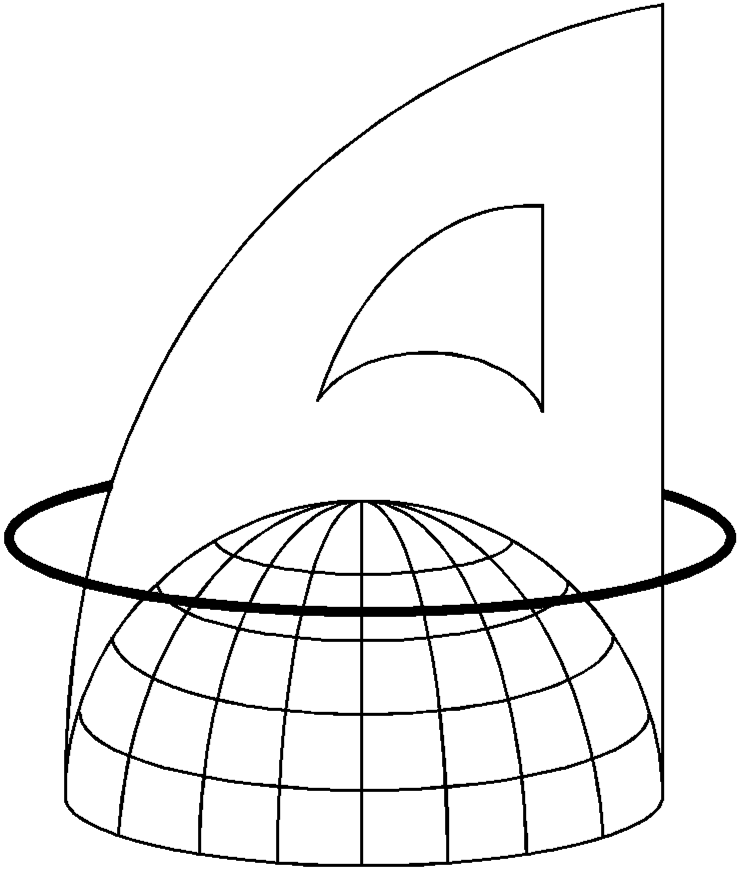
\includegraphics[width=0.4\textwidth]{logo.png}
\end{flushright}
\caption{\label{kantaratu}Albo to?}
\end{figure}

Patrzcie Państwo na Rysunek \ref{logo}, \ref{almu} oraz \ref{kantaratu}!



\end{document}

A tego już nie będzie widać!